\RequirePackage{luatex85}
\documentclass{standalone}
\thispagestyle{empty}
\usepackage{tikz}
\usepackage[compat=1.1.0]{tikz-feynman}
\begin{document}
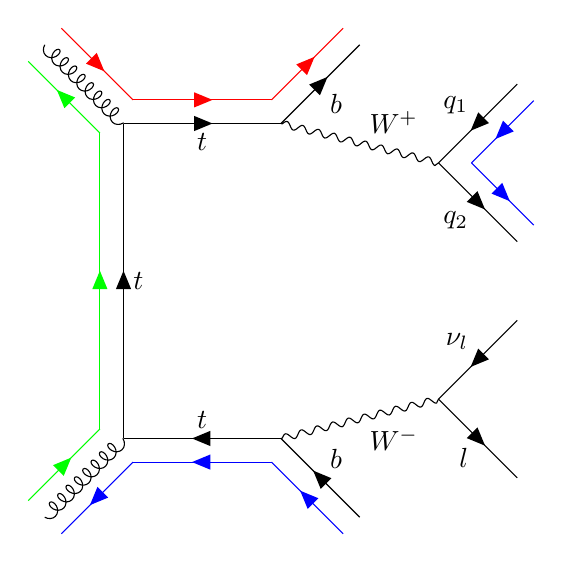
\begin{tikzpicture}
  \coordinate (delta) at (0.0, 0.3);
  \begin{feynman}
    \vertex (it);
    \vertex [below=6cm of it](ib);
    \vertex [below right=1cm and 1cm of it](t1t);
    \vertex [right=2cm of t1t](t2t);
    \vertex [above right=1cm and 1cm of t2t] (bt);
    \vertex [below right=0.5cm and 2.0cm of t2t] (Wt);
    \vertex [above right=1cm and 1cm of Wt] (ot1);
    \vertex [below right=1cm and 1cm of Wt] (ot2);
    
    \vertex [above right=1cm and 1cm of ib](t1b);
    \vertex [right=2cm of t1b](t2b);
    \vertex [below right=1cm and 1cm of t2b] (bb);
    \vertex [above right=0.5cm and 2.0cm of t2b] (Wb);
    \vertex [above right=1cm and 1cm of Wb] (ob1);
    \vertex [below right=1cm and 1cm of Wb] (ob2);
    
    \vertex (itc) at ($(it) + (0.21, 0.21)$);
    \vertex (t1tc) at ($(t1t) + (0.12, 0.3)$);
    \vertex (t2tc) at ($(t2t) + (-0.12, 0.3)$);
    \vertex (btc) at ($(bt) + (-0.21, 0.21)$);

    \vertex (ibc) at ($(ib) + (0.21, -0.21)$);
    \vertex (t1bc) at ($(t1b) + (0.12, -0.3)$);
    \vertex (t2bc) at ($(t2b) + (-0.12, -0.3)$);
    \vertex (bbc) at ($(bb) + (-0.21, -0.21)$);

    \vertex (itci) at ($(it) + (-0.21, -0.21)$);
    \vertex (t1tci) at ($(t1t) + (-0.3, -0.12)$);
    \vertex (t1bci) at ($(t1b) + (-0.3, 0.12)$);
    \vertex (ibci) at ($(ib) + (-0.21, 0.21)$);

    \vertex (ot1c) at ($(ot1) + (0.21, -0.21)$);
    \vertex (Wtc) at ($(Wt) + (0.42, 0)$);
    \vertex (ot2c) at ($(ot2) + (0.21, 0.21)$);
    \diagram*
        {
          (it) -- [gluon] (t1t),
          (t1t) -- [fermion, edge label'=\(t\)] (t2t),
          (t2t) -- [fermion, edge label'=\(b\)] (bt),
          (t1b) -- [fermion, edge label'=\(t\)] (t1t),
          (t2t) -- [boson, edge label=\(W^{+}\)] (Wt),
          (ot1) -- [fermion, edge label'=\(q_{1}\)] (Wt),
          (Wt) -- [fermion, edge label'=\(q_{2}\)] (ot2),
          (ib) -- [gluon] (t1b),
          (t2b) -- [fermion, edge label'=\(t\)] (t1b),
          (bb) -- [fermion, edge label'=\(b\)] (t2b),
          (t2b) -- [boson, edge label'=\(W^{-}\)] (Wb),
          (ob1) -- [fermion, edge label'=\(\nu_{l}\)] (Wb),
          (Wb) -- [fermion, edge label'=\(l\)] (ob2),
          (itc) -- [fermion, red] (t1tc) -- [fermion, red] (t2tc) -- [fermion, red] (btc),
          (bbc) -- [fermion, blue] (t2bc) -- [fermion, blue] (t1bc) -- [fermion, blue] (ibc),
          (ibci) -- [fermion, green] (t1bci) -- [fermion, green] (t1tci) -- [fermion, green] (itci),
          (ot1c) -- [fermion, blue] (Wtc) -- [fermion, blue] (ot2c),
        };
 %       \draw[->, red]  ($(it) + (0.0, 0.3)$) -- ($(t1t) + (0.0, 0.3)$) -- ($(t2t) + (0.0, 0.3)$);
        %\draw[->, red]  ($(t1t) + (0.0, 0.3)$) -- ($(t2t) + (0.0, 0.3)$);
        %\draw[->, red]  ($(t2t) + (0.0, 0.3)$) -- ($(bt) + (0.0, 0.3)$);

  \end{feynman}
\end{tikzpicture}
\end{document}
